\chapter*{Findings}
\begin{table}[htb]
    \renewcommand{\arraystretch}{1.5}
    \begin{tabular*}{\textwidth}{|>{\columncolor{orange!15}}p{3cm}|p{17.1cm}|}
    \textbf{Finding} & \textbf{Insecure coding leads to disk-image access}\\
    
	&\\
	Description& After researching several methods the tool 'pycdc' worked for this specific file. Inside the decompiled file an encrypted configuration was found (see attachment \ref{sec:attachment1}). Luckily the file included the private key to decrypt the configuration. The cipher used is fernet. The following script decrypted the encrypted configuration:

    \begin{lstlisting}[language=python]
#! /usr/bin/python
from cryptography.fernet import Fernet
key = b'dGH1BR5gJ6wz6rneOkvmW50UsgY_J3kBZlRIUmsSiYw='

f = Fernet(key)

token=b'gAAAAAB6U1FZADONUKESIJFYDrY8jeRSFL2TqYpqfIiTrTP8ceGBoffIZt7X
vWS5pXWE9afjswEi_fSq9D-tcEnh8QflWQu2j4158VrbjbD1s8kWRqcv665XHDiFSED
PAL1yb2w=='

decrypted f.decrypt(token)

print(decrypted)


\end{lstlisting}
    The output of the script is: 
    \begin{lstlisting}[language=python]
b'{"debug": false "initial_passphrase":"Q99mjPp4xMwnEpgJd4kd5LNe",
"mapper_name": "fde", "source_dev": "/srv/container.img",
"interface_mac": "eth0", "source_files": [["/proc/cpuinfo",  "filter_cpuinfo"],  ["/sys/kernel/debug/bluetooth/hci0/identity",  null], ["/sys/devices/platform/soc/3f980000.usb/usb1/1-1/1-1.1 /1-1.1
:1.0/net/eth0/address", null]]}'
\end{lstlisting}

From the output it can be extracted that ''debug'' is set to ''false''. By examining the decompiled file we found out that the passphrase of the container image gets printed when ''debug'' is set to ''true''. Owning the key of the fernet encryption it was possible to encrypt the same configuration we just decrypted while setting ''debug'' to ''true'' instead of ''false''. The tool vim now enables the exchange of the old encrypted configuration with the new one while the debug mode is set to true and still maintains the magic bytes of the compiled python file. After those changes the file was executed and had the following output including the passphrase of the encrypted container:
\newline
\newline
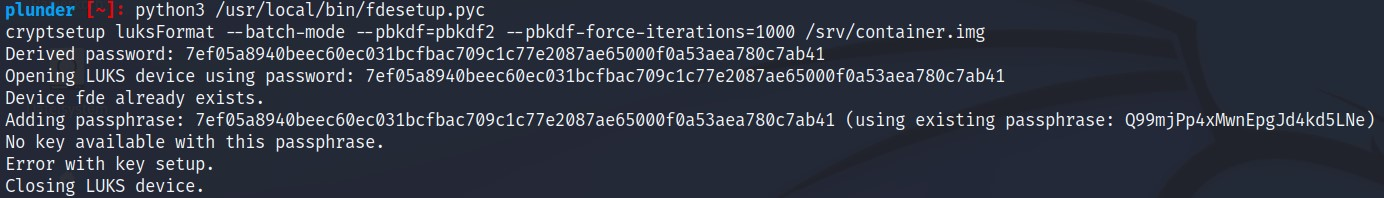
\includegraphics[width=0.85\textwidth]{passphrase.jpg}
\newline
\newline
With the given output from above we were able to access the container image.
\\
    \end{tabular*}
    \end{table}